\documentclass[paper=a4, fontsize=11pt]{scrartcl} % A4 paper and 11pt font size
\usepackage[utf8]{inputenc}
% \usepackage[german]{babel} 

% for bibtex
\usepackage{cite}

\usepackage{amsmath,amsfonts,amsthm} % Math packages
\newcommand{\norm}[1]{\left\lVert#1\right\rVert} 

\usepackage{amssymb}
\usepackage{amsthm}

\usepackage{graphicx}
\usepackage{svg}
\usepackage{import}
\usepackage{siunitx}
\usepackage{minted}

\usepackage{url}
\usepackage{sectsty} % Allows customizing section commands


\usepackage{titlesec}

% center section titles and omit numbering
% \titleformat{\section}[block]{\Large\bfseries\filcenter}{}{1em}{}



\usepackage{tikz}
\usepackage{fancyhdr} % Custom headers and footers
\pagestyle{fancyplain} % Makes all pages in the document conform to the custom headers and footers
\fancyhead{} % No page header - if you want one, create it in the same way as the footers below
\fancyfoot[L]{} % Empty left footer
\fancyfoot[C]{} % Empty center footer
\fancyfoot[R]{\thepage} % Page numbering for right footer
\renewcommand{\headrulewidth}{0pt} % Remove header underlines
\renewcommand{\footrulewidth}{0pt} % Remove footer underlines


\setlength{\headheight}{13.6pt} % Customize the height of the header
\setlength{\parskip}{0.5em}
\setlength{\parindent}{0em}

\numberwithin{equation}{section} % Number equations within sections (i.e. 1.1, 1.2, 2.1, 2.2 instead of 1, 2, 3, 4)
\numberwithin{figure}{section} % Number figures within sections (i.e. 1.1, 1.2, 2.1, 2.2 instead of 1, 2, 3, 4)
\numberwithin{table}{section} % Number tables within sections
% \item
% \item (i.e. 1.1, 1.2, 2.1, 2.2 instead of 1, 2, 3, 4)


\newtheorem{mydef}{Definition}


\title{Relations between spatial objects} 
\author{Simon Fromme}

\date{\normalsize edited on \today}

\begin{document}

\maketitle
\newpage
\tableofcontents
\newpage

\section{Motivation}
In recent years 3D geo data becomes increasingly available and more and more cities decided to create digital 3D models of their building stock. This development was aided by many public agencies commissioning laser-scanning (LiDAR) and photogrammetry of their territories with the so deduced data oftentimes serving as a basis for 3D city models. Besides buildings city models often also include entities such as infrastructure objects (e.g. tunnels, bridges), city furniture (e.g. monuments, fountains) and vegetation thus providing a basis for a variety of potential applications based on 3D spatial data.

Conceivable projects based on the data provided by 3D city models include among others:
\begin{itemize}
\item visibility analysis, e.g. predicting whether the construction of a high-rise building would block the view to a historic church from certain apartments
\item shadow analysis, e.g predicting the location and intensity of cast shadows in the planning phase of a new skyscraper
\item visualization of new buildings in a realistic environment prior to construction
\item illumination simulations (e.g. for the illumination of historic churches or castles)
\item calculation of the solar energy potential for entire areas
\item noise and pollutant predictions (e.g. the implications of a new urban freeway on the noise level in surrounding neighborhoods may be computed using the data of a city model).
\end{itemize}

To facilitate some of these tasks it would oftentimes be of great help to have a spatial query language that allowed for standardized spatial requests to carry out common tasks such as
\begin{itemize}
\item retrieve all spatial entities that are in a 300 meter radius of a certain building,
\item retrieve all buildings that are directly connected to a certain building or
\item retrieve all residential buildings west of an exhaust emitting factory.
\end{itemize}

However, at the moment of this writing no established query language is known to the author that allows for complex queries based on the geometry of spatial entities (in particular building models) in 3D. Most query languages only take into account relations explicitly modeled in the language the feature was modeled in but don't take into account the information implicitly given by the geometry.  

\section{Purpose}
The purpose of this work is to investigate spatial relations based explicitly on the geometry of geographic features. This means that all geometries are referenced in a geographic coordinate system thus have a definite position and orientation in space. 

In a first step (section \ref{sec:types-geom-relat}) general aspects and previous work on spatial relations are examined. This includes both the formal definition and the underlying models needed for an actual implementation of a program that can decide whether the defined relation holds \emph{true} or \emph{false}. 

In this section and in the whole course of this work three kinds of spatial relations are distinguished:
\begin{enumerate}
\item  \emph{Topological} (section \ref{sec:topol-relat-1}),
\item \emph{Metric} (section \ref{sec:metric-relations-1}) and
\item \emph{Directional} relations (section \ref{sec:directional-relations} ).
\end{enumerate}

In section \ref{sec:implementation} the programmatic implementation of a number of spatial relations between geographical features is presented. For this purpose a Ruby program was written that is capable of
\begin{itemize}
\item building up an index of geographical features from a CityGML-file by parsing and subsequently converting individual buildings into a custom data model,
\item computing all features from the spatial index for which a specific spatial relation holds true relative to a specified feature,
\item providing access to the spatial index by means of a REST API. Return formats include XML and KMZ (Google Earth) and 
\item providing an interface by means of a REST API to allow for the retrieval of those features for which a specific spatial relation holds true, provided a reference feature for the relation is specified. \end{itemize}

The choice and the actual implementation of the supported spatial relations are discussed in the sections \ref{sec:topol-relat}, \ref{sec:metric-relations} and \ref{sec:direct-relat}. Since a requirement for the program was to return the resulting dataset as a KMZ-file at request to allow for rendering of the feature geometries in Google Earth, a number of difficulties has to be addressed also described in section \ref{sec:implementation}.  

The program and Web API were tested using a subset of the 3D city model of the city of Karlsruhe in CityGML as an input. This model was kindly provided by the real estate office (``Liegenschaftsamt'') of the city of Karlsruhe in LoD\footnote{LoD = ``Level of Detail'', see section \ref{sec:input-datasets} for more detailed information} 2. As the city model contains 1685 individual buildings the runtime of parsing, the computation of spatial relations and the generation of output files became an issue. Since the implementation did not focus on performance a short analysis of the status quo and possible improvements regarding runtime are discussed in section \ref{sec:performance}. 

Eventually a conclusion and an outlook are given in section \ref{sec:outlook}. 

\section{Spatial relations}\label{sec:types-geom-relat}
A spatial relation as used here is a binary relation between two real world objects with the focus on objects having dimension $d = 3$. Since we are dealing with real world objects such as houses we will only consider relation $R$ with $R \subseteq \mathbb{R}^3\times \mathbb{R}^3$ assuming a real world object can be considered subsets of $\mathbb{R}^{3}$.

Commonly three types of spatial relations are distinguished, that are
\begin{enumerate}
\item  \emph{Topological} (section \ref{sec:topol-relat-1}),
\item \emph{Metric} (section \ref{sec:metric-relations-1}) and
\item \emph{Directional} relations (section \ref{sec:directional-relations} ).
\end{enumerate}
Each relation category will be reviewed taking into consideration a formal definition, underlying models for an implementation and possible applications. 

Spatial relations that do not fall in either of the three categories such as \emph{``close to''}, \emph{``about 10 km southwest of''} (approximate relations) or \emph{``into''} (relation depending on the motion of an object) will not be considered here.

For real world use one often only wants to deal with only a certain set of (theoretically infinite) possible relations. Also one wants to assign names to relations that are understandable by humans but still needs to make sure these relations are defined unambiguously on a formal level which is not always the case for solely linguistic. E.g. its is not clear what is meant exactly meant when saying an object is located \emph{``west''} of some other object.

This poses the problems of 
\begin{enumerate}
\item the identification of a set of spatial relations that is small enough to be reasonably used in an application and yet is big enough to not lose expressiveness,n
\item finding a formal definition for a relation that complies with the name of the relation in natural language and
\item determining a model for the actual implementation of the specific relation depending on the data structure in which the spatial objects are given. 
\end{enumerate}

These will be addressed in the following sections.


\subsection{Topological relations}\label{sec:topol-relat-1}
The characteristic that distinguish topological relations from other kinds of relations is that they are preserved under topological transformations (continuous maps) of the involved objects. These transformations include e.g.
\begin{itemize}
\item \emph{translation},
\item \emph{rotation} and
\item \emph{scaling}.
\end{itemize}
Hence topological relations do not depend on the size or orientation of the involved objects in space but merely on what would casually be called their connection. For example two objects would be considered neighbors if they share a common boundary. The relation ``A is neighbor of B'' would not depend on the size nor the orientation of this boundary. Examples of topological relations would be \emph{insideOf}, \emph{touching} and  \emph{intersecting}.

In an abstract sense a continuous map $f:X \rightarrow Y$ between two topological spaces $X$ and $Y$, requires the preimage of any open set in $Y$ to be an open set in $X$. Given a binary relation $T\subseteq X\times X$ between sets in $X$ the relation would be unchanged if these set would undergo a transformation $f$ first.

Since we will be dealing with real world objects rather than subsets in abstract topological spaces we will from now on consider only topological relations $T\subseteq \mathbb{R}^n \times \mathbb{R}^n$ with $n$ being $1$,$2$ or $3$ depending on what dimension the involved objects have.

Possible applications that would make use of querying based on topological relations in a building context would be:
\begin{itemize}
\item querying for all rooms \emph{``inside of''} a building (if those are modeled as separate entities), e.g. to quickly calculate the amount of color needed to paint them.
\item querying for \emph{intersecting} building geometries in two different building data that partially overlap to identify duplicates.
\item identify all buildings of a building block by querying for making use of subsequent \emph{``is touching''} queries.
\end{itemize}

\subsubsection{Prerequisites}\label{sec:prerequisites-1}
As a prerequisite for the following sections a number of definitions are given that can also be found in most elementary text books on topology and multidimensional analysis.

Let $A$ be a subset of $\mathbb{R}^3$.


\textbf{Interior}\\
The interior of a set $A$ is denoted by $A^{\circ}$. It is the union of all open subsets of $A$ and hence is a subset of $A$ itself. It is formally defined as
\begin{align*}
  A^o := \{ x\in \mathbb{R}^3  : \exists \epsilon > 0 : U_{\epsilon}(x) \subseteq A \},
\end{align*}
where $U_{\epsilon}(x_0) = \{ x \in \mathbb{R}^n : \norm{x-x_0}_2< \epsilon \}$ is the unit sphere around $x_0$. 
That means that for every point $x$ in $A^o$ there exists some arbitrary small sphere around $x$ that is still entirely inside of $A$. 

\textbf{Boundary} \\
The boundary of a set A is denoted by $\partial A$ and is formally defined as
\begin{align*}
  \partial A := \{ x \in \mathbb{R}^3 : \forall \epsilon > 0 : U_{\epsilon}(x) \cap A \ne \varnothing \wedge U_{\epsilon}(x) \cap (\mathbb{R}^3 \setminus A) \ne \varnothing    \}.
\end{align*}
The idea of this definition is that an arbitrary small sphere around a point in $\partial A$ intersects with both the set $A$ and its exterior $(\mathbb{R}^3 \setminus A)$.

When an object is represented in BRep the boundary $\partial A$ is thus equal to the given $n-1$ dimensional shell.  

\textbf{Exterior} \\
The exterior of a set $A$ is equivalent to the complement of $A$ denoted by $A^c$. Thus it holds
\begin{align*}
  A^c:=\{x\in \mathbb{R}^3:x\notin A\}
\end{align*}

\begin{figure}
  \centering
  \def\svgwidth{15em}
  \import{img/}{topology.eps_tex}
  \caption{the set $A \subset \mathbb{R}^2$ together with its interior $A^{\circ}$, boundary $\partial A$ and exterior $A^c$}
  \label{fig:mbr}
\end{figure}

\subsubsection{The 4-Intersection Model}\label{sec:4-intersection-model}
To formalize topological relations between spatial objects different approaches were taken, one being the 4-Intersection Model which was later extended to a 9-Intersection Model. Since the latter will be used here it will be discussed in the following section.

The 4-Intersection Model (4-IM) was described by M. J. Egenhofer and R. Franzosa in 1991 \cite{Egenhofer:1991:IJGIS} and makes use of point set theory. The idea is to treat objects as sets in a topological space (here $X = \mathbb{R}^3$) and to examine a $2\times 2$ matrix composed of the mutual intersections of the objects interiors and boundaries that is defined as
\begin{align*}
  I := \begin{pmatrix}
    A^{o} \bigcap B^{o}        & A^{o} \bigcap \partial B  \\
    \partial A \bigcap B^{o}  & \partial A \bigcap \partial B  \\
  \end{pmatrix}.
\end{align*}
As each matrix element can either be empty ($\varnothing$) or non-empty ($\neg\varnothing$), $2^4 = 16$ different configuration of the matrix are possible. Eight of those configurations are identified as predicates that occur in real situations. For objects in 2D Egenhofer identifies eight possible relations depicted in Figure \ref{fig:4im}.

\begin{figure}[!h]
  \centering  
  \def\svgwidth{\textwidth}
  \import{img/}{4IM.eps_tex}
  \caption{topological relations in 2D as distinguished by the 4-Intersection Model}
  \label{fig:4im}
\end{figure}

with the corresponding 4IM matrices:

\begin{align*}
\begin{pmatrix}
    \varnothing & \varnothing \\
    \varnothing & \varnothing \\
  \end{pmatrix}, 
  \begin{pmatrix}
    \neg\varnothing & \neg\varnothing \\
    \varnothing & \varnothing \\
  \end{pmatrix}, 
  \begin{pmatrix}
    \neg\varnothing & \varnothing \\
    \neg\varnothing & \varnothing \\
  \end{pmatrix}, 
  \begin{pmatrix}
    \neg\varnothing & \varnothing \\
    \varnothing & \neg\varnothing \\
  \end{pmatrix}, 
  \begin{pmatrix}
    \varnothing & \varnothing \\
    \varnothing & \neg\varnothing \\
  \end{pmatrix}, 
  \begin{pmatrix}
    \neg\varnothing & \neg\varnothing \\
    \varnothing & \neg\varnothing \\
  \end{pmatrix}, 
  \begin{pmatrix}
    \neg\varnothing & \varnothing \\
    \neg\varnothing & \neg\varnothing \\
  \end{pmatrix}, 
  \begin{pmatrix}
    \neg\varnothing & \neg\varnothing \\
    \neg\varnothing & \neg\varnothing \\
  \end{pmatrix}. 
\end{align*}

\subsubsection{The 9-intersect model}



\subsubsection{Metric Relations}\label{sec:metric-relations-1}



\subsection{Directional Relations}\label{sec:directional-relations}

Another kind of relation to distinguish are relations that take into considerations the relative directions between objects. Intuitive examples are predicates like \emph{left}, \emph{right}, \emph{above}, \emph{below}, \emph{eastOf}, ...

In the context of city models one might be interested in all buildings west of an exhaust emitting factory, since that is the prefered wind direction in central europe. A geometry based query for bridges might be based on the \emph{above} relationship relative to a specified street and one might want to verify the statement that riverbanks on the northern hemisphere erode more on the right handside relative to the direction of flow by querying for objects on this side of the river. 

To decide whether a specific directional relation holds or to find all objects that are related to a given object in terms of a given relation with computational means, it is necessary to clearly define

\begin{enumerate}
\item a \emph{set of relations} to be supported by the program and
\item \emph{underlying models} for these relations that the computer then uses to decide whether a relation does hold or not in a given spatial context. 
\end{enumerate}

For both questions a number of approaches exist, some of them presented in this work in a first step. 

\subsubsection{formal definition}

When speaking about directional relations it is important to specify a reference frame relative to which these relations are being considered. Following \cite{Retz-Schmidt:1988:VVS:46184.46189} Borrmann and Rank \cite{Borrmann:2009:AEI} distinguish three different kinds of reference frames, namely
\begin{itemize}
\item an \emph{intrincic} reference frame that is the defined by the inner orientation of the object such as the front side of a house or the right side of a river relative to the flow,
\item a \emph{deitic} a reference frame that is dependent on the position of an external observer and 
\item an \emph{extrinsic} reference frame that is defined by some external reference points. 
\end{itemize}

Taking into account the different meaning of the predicates \emph{left} and \emph{right} in a reference frame relative to an observer or relative to the frontside of a building it becomes clear that a reference frame must be specified when using either of those predicates.

We thus define a directional relation as a tuple $(D,RF)$ where  
\begin{align*}
  D \subseteq A \times B 
\end{align*}
with $A$ and $B$ being sets of objects and $RF$ a reference frame.

Since directional relationships can be defined unambiguously only for point sized objects it is necessary to work out models to define those relations for spatially extended objects in higher dimensions. 

Borrmann and Rank \cite{Borrmann:2009:AEI} list a number of previous approaches that were developed to address this problem for objects with at least one having dimension 1 or above.

\subsubsection{previous work}\label{sec:previous-work}
The most simple yet common approach is to use an objects center of gravity (or some other distinguished point) and to define directional relations between spatially extended objects as 0D-0D-relationships between those points. This is easy and unambiguous, however, it sometimes yields counter intuitive results as seen in Figure \ref{fig:center_gravity} where the center of gravity of $B$ is \emph{above} the center of gravity of $A$ although a person would probably classify the relationship the other way around. Thus using this simple approach might be easy to implement but sometimes lacks significance in complex scenarios.

\begin{figure}
  \centering
  % \includegraphics[width=3cm]
  \def\svgwidth{10em}
  \import{img/}{center_gravity.eps_tex}
  \caption{counter intuitive result when defining directional relations via the centers of gravity. The relation ``$B$ is \emph{above} $A$'' would hold in this case although that certainly violates common opinion.  }
  \label{fig:center_gravity}
\end{figure}

In a two-dimensional space Borrmann and Rank \cite{Borrmann:2009:AEI} distinguish two different approaches to define directional relations between point size objects: the \textit{cone-based} and the \textit{direction-based} model. 

% TODO: insert original references for this model
In the cone-based model the space around a point gets dissected into a number of equally sized partitions (usually 4 or 8) and the direction of a target point from 

\begin{figure}
  \centering
  \def\svgwidth{15em}
  \import{img/}{direction_cone_model_4.eps_tex}
  \caption{According to the cone-based model in 2D-space the point B is located \emph{eastOf} the point A.}
  \label{fig:direction_cone_model_4}
\end{figure}

In the direction-based model the space is divided into a northern and southern and an eastern and western halfspace relative to some reference point respectively. By projecting a target point on each pair of halfspaces one gets the four possible directions: \emph{northEastOf}, \emph{southEastOf}, \emph{southWestOf} and \emph{northWestOf}. 

A different approach to define directional relations between 2D objects is to use their minimum bounding rectangle (MBR) representation.

\begin{mydef}
  A minimum bounding rectangle (MBR) is a rectangle, oriented to the x- and y-axes, that bounds a geographic feature or a geographic dataset. It is specified by two coordinate pairs: $x_{\mathrm{min}}$, $y_{\mathrm{min}}$ and $x_{\mathrm{max}}$, $y_{\mathrm{max}}$.\footnote{definition according to \url{http://en.mimi.hu/gis/minimum_bounding_rectangle.html}}
\end{mydef}

Given the MBR of two objects: ($x^{(1)}_{\mathrm{min}}$, $y^{(1)}_{\mathrm{min}}$, $x^{(1)}_{\vphantom{\mathrm{i}}\mathrm{max}}$, $y^{(1)}_{\vphantom{\mathrm{i}}\mathrm{max}}$) and ($x^{(2)}_{\mathrm{min}}$, $y^{(2)}_{\mathrm{min}}$, $x^{(2)}_{\vphantom{\mathrm{i}}\mathrm{max}}$, $y^{(2)}_{\vphantom{\mathrm{i}}\mathrm{max}}$) one examines the projections onto the x- and y-axis of each bounding boxe and uses the characterization of 1D interval relations between $[x^{(1)}_{\mathrm{min}}, x^{(1)}_{\vphantom{\mathrm{i}}\mathrm{max}}]$, $[x^{(2)}_{\mathrm{min}}, x^{(2)}_{\vphantom{\mathrm{i}}\mathrm{max}}]$ and $[y^{(1)}_{\mathrm{min}}, y^{(1)}_{\vphantom{\mathrm{i}}\mathrm{max}}]$, $[y^{(2)}_{\mathrm{min}}, y^{(2)}_{\vphantom{\mathrm{i}}\mathrm{max}}]$ respectively. 

Having defined $n$ relations between 1D intervals one obtains $n^d$ interval relations in a $d$-dimensional space that can then be used to define directional relations between the two objects. 

Allen \cite{Allen:1983:MKT:182.358434} classifies 13 relations between (originally temporal) intervals in a 1D space, such as \textit{Interval $I_1$ is before Interval $I_2$} or \textit{$I_1$ overlaps $I_2$} that are used by other authors for classifications of 1D relationships. Out of those relations Guesgen \cite{guesgen1989spatial} uses a set of eight (\emph{left}, \emph{attached}, \emph{overlapping}, \emph{inside} and the reversed versions) to describe to and formally reason about spatial relationships in more-dimensional models. This is done by means of $d$-dimensional relationship tuples, since each dimension is considered to be independent from the others. 

An example of this method is pictured in Figure \ref{fig:mbr}. If one sticks to the interval relations proposed by Guesgen one would describe the relations of $A$ to $B$ as the tuple (\emph{above}, \emph{overlapping}) where the first tuple entry refers to the x- and the second one to the y-direction. However, the \emph{overlapping} predicate is considered to be rather a topological relation in this thesis. 

\begin{figure}
  \centering
  \def\svgwidth{20em}
  \import{img/}{mbr.eps_tex}
  \caption{Using minimum bounding rectangles to define directional relations in 2D. The MBRs are projected on both the x- and y-axis. Subsequently one-dimensional relations between the projection intervals $I^{(1)}_x$, $I^{(2)}_x$  and $I^{(1)}_y$, $I^{(2)}_y$ are evaluated independently and are then combined in a tuple.}
  \label{fig:mbr}
\end{figure}

Papadias et al. \cite{papadias1995topological} use the whole set of Allen's 13 relations thus obtaining 169 relations in 2D but a distinction between topological and directional relations is not being made. 

Borrmann also mentions a model by Goyal \cite{goyal2000similarity} that parts the space around a reference object on the basis of its MBR and introduces a matrix that records in which segments a target object falls. This is easily extendable to three dimensions, however, Goyal does not assign names to the different matrix configurations making it unsuitable for a spatial query language.  

Coming to the conclusion that little work has been put into developing models on directions in 3D space Borrmann \cite{Borrmann:2009:AEI} proposes two new models:  the \textit{projection based} and the \textit{half space model}. 


\paragraph{the projection-based directional model}\label{sec:proj-based-direct}
Both models are suited for objects of any dimensions. Spatial relations are examined separately for each axis, thus no combined relations such as \emph{northEastOf} is being computed. In three dimensions six distinct relations are part of the model:
\begin{table}[h!]
  \begin{tabular}{cl}
    \textbf{axis} & \textbf{relations} \\
    x  & \emph{northOf}, \emph{southOf} \\
    y  & \emph{eastOf}, \emph{westOf} \\
    z  & \emph{above}, \emph{below}
  \end{tabular}
\end{table}

The idea is to extrude the reference object in the direction of one axis (e.g. the x-axis for the \emph{northOf} relation) and to check for intersections with the extrusion. Borrmann distinguishes a relaxed and a strict version of these relations. For the ``relaxed'' version to hold it is sufficient for a target object to intersect with the extrusion of the reference object in the respective direction. For the ``strict'' version it is necessary for the target object to lay fully inside of the extrusion on the respective side of the axis. 

\begin{figure}
  \centering
  \def\svgwidth{20em}
  \import{img/}{direction-model.eps_tex}
  \caption{direction-based model: According to the relaxed version of the \emph{above} relation the cubes $B$, $C$ and $D$ would be considered to be \emph{above} the gray object. According to the strict version only the cubes $B$ and $C$ would be. }
  \label{fig:direction-model}
\end{figure}


This can be formalized in the following way. 

%% TODO: provide graphic for further explanation

\textbf{relaxed}
\begin{align*}
  \mathrm{eastOf\_proj\_relaxed}(A,B) :\Leftrightarrow \exists a,b:a_y=b_y\wedge a_z=b_z\wedge a_x<b_x, \\
  \mathrm{westOf\_proj\_relaxed}(A,B) :\Leftrightarrow \exists a,b:a_y=b_y\wedge a_z=b_z\wedge a_x>b_x, \\
  \mathrm{northOf\_proj\_relaxed}(A,B) :\Leftrightarrow \exists a,b:a_x=b_x\wedge a_z=b_z\wedge a_y<b_y, \\
  \mathrm{southOf\_proj\_relaxed}(A,B) :\Leftrightarrow \exists a,b:a_x=b_x\wedge a_z=b_z\wedge a_y>b_y, \\
  \mathrm{above\_proj\_relaxed}(A,B) :\Leftrightarrow \exists a,b:a_x=b_x\wedge a_y=b_y\wedge a_z<b_z, \\
  \mathrm{below\_proj\_relaxed}(A,B) :\Leftrightarrow \exists a,b:a_x=b_x\wedge a_y=b_y\wedge a_z>b_z. \\
\end{align*}

\textbf{strict}\footnote{It has to be noted that Borrmann made a mistake in his original publication \cite{Borrmann:2009:AEI} where at some points he mistakenly exchanged $a$ for $b$ in the definitions of the ``strict'' relations for the projection-based directional model. These rather apparent mistakes were corrected here.} 
\begin{align*}
  \mathrm{eastOf\_proj\_strict}(A,B) :\Leftrightarrow \forall b:&(\exists a:a_y=b_y\wedge a_z=b_z\wedge a_x<b_x) \wedge \\&(\not\exists a:a_y=b_y\wedge a_z=b_z\wedge a_x\ge b_x), \\
  \mathrm{westOf\_proj\_strict}(A,B) :\Leftrightarrow \forall b:&(\exists a:a_y=b_y\wedge a_z=b_z\wedge a_x>b_x) \wedge \\&(\not\exists a:a_y=b_y\wedge a_z=b_z\wedge a_x\le b_x), \\
  \mathrm{northOf\_proj\_strict}(A,B) :\Leftrightarrow \forall b:&(\exists a:a_x=b_x\wedge a_z=b_z\wedge a_y<b_y) \wedge \\&(\not\exists a:a_x=b_x\wedge a_z=b_z\wedge a_y\ge b_y), \\
  \mathrm{southOf\_proj\_strict}(A,B) :\Leftrightarrow \forall b:&(\exists a:a_x=b_x\wedge a_z=b_z\wedge a_y>b_y) \wedge \\&(\not\exists a:a_x=b_x\wedge a_z=b_z\wedge a_y\le b_y), \\
  \mathrm{above\_proj\_strict}(A,B) :\Leftrightarrow \forall b:&(\exists a:a_x=b_x\wedge a_y=b_y\wedge a_z<b_z) \wedge \\&(\not\exists a:a_x=b_x\wedge a_y=b_y\wedge a_z\ge b_z), \\
  \mathrm{above\_proj\_strict}(A,B) :\Leftrightarrow \forall b:&(\exists a:a_x=b_x\wedge a_y=b_y\wedge a_z>b_z) \wedge \\&(\not\exists a:a_x=b_x\wedge a_y=b_y\wedge a_z\le b_z).
\end{align*}

\paragraph{the half-space based model}\label{sec:half-space-based-model}
In the half-space based model one does not consider the extrusion of an object but the entire half space in one direction when checking for intersection of the target with the reference object. If the target object lays completely inside the half-space (e.g. above an object) one considers the ``strict''  version of the relation to hold. 

In the ``relaxed'' version one does also allow for intersections of the target with the reference object requiring only part of the object to lay further in the direction of the specific relation. 

\begin{figure}
  \centering
  \def\svgwidth{20em}
  \import{img/}{hf-model.eps_tex}
  \caption{half-space based model: According to the relaxed version of the \emph{above} relation the cubes $A$, $B$ and $C$ would be considered to be \emph{above} the gray object. According to the strict version only the cubes $A$ and $B$ would be. \\ In contradiction to the direction based model $C$ would not be considered to be \emph{above} (relaxed/strict) the gray object }
  \label{fig:direction-model}
\end{figure}

\textit{\textbf{Example}: For the relation ``$B$ above\_hs\_relaxed $A$'' to hold it is necessary that for every point of $A$ there is at least one point of $B$ with a greater z-component. 
}

Borrmann consecutively arrives at the following formal definitions:


\textbf{relaxed-version}
\begin{align*}
  \mathrm{eastOf\_hs\_relaxed}(A,B) :\Leftrightarrow \exists b: \forall a: a_x<b_x,  \\
  \mathrm{westOf\_hs\_relaxed}(A,B) :\Leftrightarrow \exists b: \forall a: a_x>b_x,  \\
  \mathrm{northOf\_hs\_relaxed}(A,B) :\Leftrightarrow \exists b: \forall a: a_y<b_y, \\
  \mathrm{southOf\_hs\_relaxed}(A,B) :\Leftrightarrow \exists b: \forall a: a_y>b_y, \\
  \mathrm{above\_hs\_relaxed}(A,B) :\Leftrightarrow \exists b: \forall a: a_z<b_z,   \\
  \mathrm{below\_hs\_relaxed}(A,B) :\Leftrightarrow \exists b: \forall a: a_z>b_z.
\end{align*}
and
\textbf{strict-version}
\begin{align*}
  \mathrm{eastOf\_hs\_strict}(A,B) :\Leftrightarrow \forall a,b: a_x<b_x,  \\
  \mathrm{westOf\_hs\_strict}(A,B) :\Leftrightarrow \forall a,b: a_x>b_x,  \\
  \mathrm{northOf\_hs\_strict}(A,B) :\Leftrightarrow \forall a,b: a_y<b_y, \\
  \mathrm{southOf\_hs\_strict}(A,B) :\Leftrightarrow \forall a,b: a_y>b_y, \\
  \mathrm{above\_hs\_strict}(A,B) :\Leftrightarrow \forall a,b: a_z<b_z,   \\
  \mathrm{below\_hs\_strict}(A,B) :\Leftrightarrow \forall a,b: a_z>b_z. 
\end{align*}

\section{Implementation}\label{sec:implementation}

\subsection{input datasets}\label{sec:input-datasets}
As the objective of this thesis is to implement geometry-based relations for spatial, georeferenced objects the first task was to identify suitable datasets as a basis for the following computation. The most important requirements for this were as follow.
\begin{enumerate}
\item The input data should be of low complexity to reduce computational costs and to minimize efforts for parsing and mapping the input data to the chosen internal data-structure. Especially the use of raw sensor data (e.g. laser-scanning and photo-grammetry data) was considered to be disproportional for the purpose of this work.
\item The input data should be widely-used in a geospatial context to allow for the reuse of parts of the program.
\item The data format of the input data should allow for parsing with publicly available tools that are available under a suitable license. 
\end{enumerate}

An appropriate candidate that was used here is an extract of the 3D city model of Karlsruhe, Germany. The data set consists of 1625 buildings in the city center spanning an area of about $\SI{2}{\kilo\meter^2}$. Each building consists of a number of building parts (mostly roof and base body) and is represented in BRep\footnote{boundary representation: A geometry in BRep is represented by its boundary, e.g. a cube by the six squares bounding it.} with each boundary surface being a plane, convex\footnote{This characteristic allows for trivial triangulation of a polygon. If this can not be assumed, triangulation can be carried out e.g. as described by Chazelle \cite{chazelle1991} who proposed a linear time algorithm for the common case of simple polygons.  } polygon. 

The datasets file format is CityGML 2.0, which is an XML-based encoding for the representation, storage and exchange of virtual 3D city and landscape models.\footnote{\url{http://www.citygml.org/index.php?id=1523}} CityGML is an application schema of for the Geography Markup Language (GML) which is an international standard\footnote{issued by the Open Geospatial Consortium, OGC (\url{http://portal.opengeospatial.org/files/?artifact_id=4700}) and the ISO TC211 (\url{http://www.isotc211.org/}).} for the exchange of spatial data. It allows for the description of a wide range of city objects including vegetation, bridges and water bodies. CityGML is open, can be used free of charge and is used globally in various projects and software solutions. The CityGML website mentions infrastructure programs e.g. in the Netherlands, Germany, France, Malaysia and Abu Dhabi that rely on CityGML.  

CityGML allows for the representation of 3D objects in five different levels of detail (LoD) ranging from a rather imprecise representation of a region/landscape (LoD 0) to architectural models with a modeled interior (LoD 4). It is common and possible to represent a given set of objects in multiple LoDs simultaneously allowing it applications to use the most suitable representation for a given purpose. The extract of the Karlsruhe model was made available in ``LoD 2'' only for the purpose of this work by the ``Liegenschaftsamt Karlsruhe''. Individual points were represented in the Gauss-Kruger reference system (``Gauss-Kruger, zone 3'') in the particular dataset.

\begin{figure}
  \centering
  \includegraphics[width=34em]{img/city_model}
  \caption{Part of the used dataset viewed in "Aristoteles3D GML Viewer"}
  \label{fig:city_model}
\end{figure}

\begin{figure}[h]
  \centering
  \includegraphics[width=34em]{img/city_model_detailed}
  \caption{complex building in the dataset viewed in "Aristoteles3D GML Viewer"}
  \label{fig:city_model_detailed}
\end{figure}


To also include objects of a lower dimension a number of 0D points of interest in the area of the 3D city model were obtained using the SPARQL endpoint of the German DBpedia (\url{http://de.dbpedia.org/sparql}) using the following query.

\begin{minted}{sql}
  PREFIX geo: <http://www.w3.org/2003/01/geo/wgs84_pos#>
  PREFIX georss: <http://www.georss.org/georss>

  SELECT ?res (bif:st_distance(?geo, ?bb_geo))
  WHERE {
    <http://de.dbpedia.org/resource/Karlsruher_Pyramide> georss:point ?bb_geo .
    ?res  georss:point ?geo .
    FILTER (bif:st_intersects(?geo, ?bb_geo, 1000))
  } LIMIT 100
\end{minted}

Out of the returned dataset lat/long coordinates in WGS84, name and description were extracted. 

\subsection{internal data model}\label{sec:internal-data-model}
Before the actual computation of spatial relations can take place the input datasets are parsed and translated in an internal data model in a first step. As no suitable CityGML parser with Ruby bindings was available at the time of this writing, the data was extracted with the Ruby library ``Nokogiri"\footnote{\url{http://www.nokogiri.org/}}, an HTML, XML, SAX, and reader and parser based on the C-libraries ``libxml2'' and ``libxslt'', with the help of XPath expressions and CSS3 selectors. To translate WGS84 into Gauss-Kruger coordinates the bash-program ``cs2cs''\footnote{used proj4 strings for coordinate transformation: \\ \texttt{+proj=tmerc +lat\_0=0 +lon\_0=9 +k=1.000000 +x\_0=3500000 +y\_0=0 +ellps=bessel +datum=potsdam +units=m +no\_defs} (Gauss-Kruger, zone 3), \\ \texttt{+proj=longlat +ellps=WGS84 +datum=WGS84 +no\_defs} (WGS84)} that ``performs transformation between the source and destination cartographic coordinate system on a set of input points'', is invoked by the application. 

To internally represent the individual features and building geometries a simple data model was developed that allows to represent a building geometry in different dimensions (0D, 1D, 2D and 3D). 

A 0D-geometry is described by a single Point (east, north, height) in ``Gauss-Kruger, zone 3'' coordinate system which also is the fundamental entity in this model. 1D-geometries are described by a number of (connected) lines which each are represented by an ordered pair of points. 2D-geometries are modeled as a set of (simple\footnote{flat and consisting of non-intersecting lines only} and convex) polygons each represented by an ordered list of points with the first point one being equal to the last one.  Finally a 3D-geometry is modeled as a list of 3D meshed which each mesh represented by its boundary as a set of (connected) polygons. Figure \ref{fig:uml} shows an UML diagram of the chosen data model.     

\begin{figure}[h]
  \centering
  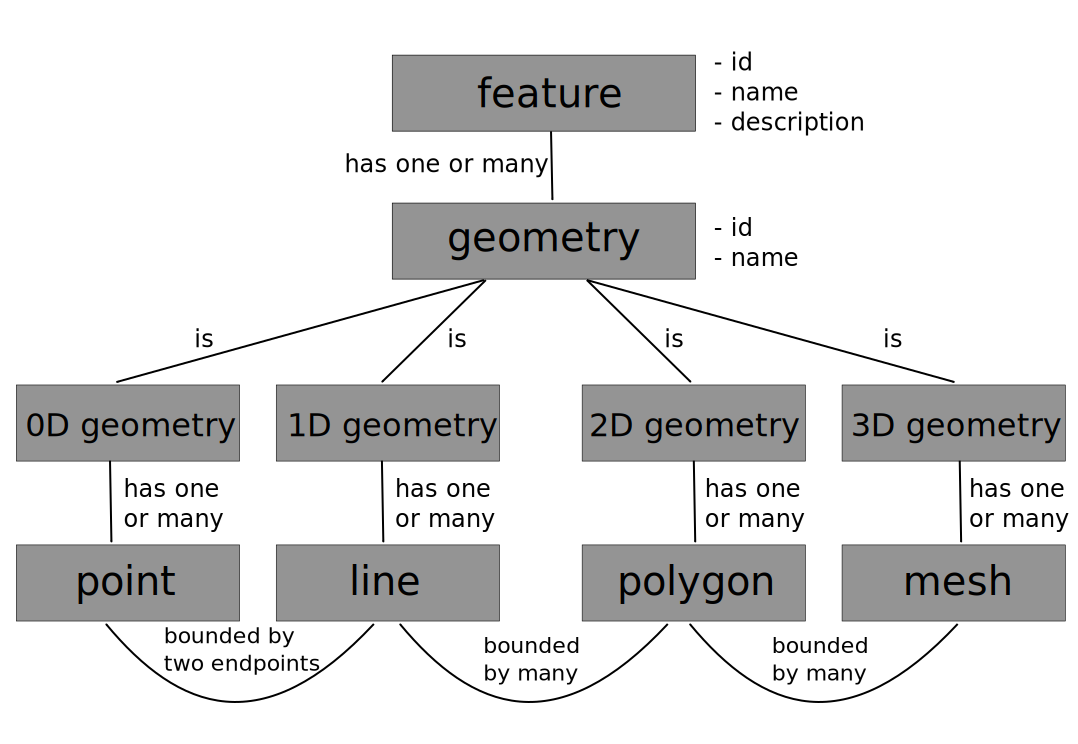
\includegraphics[width=34em]{img/uml}
  \caption{UML-diagram of the used data model to represent a feature}
  \label{fig:uml}
\end{figure}

\subsection{KML/Collada Export}\label{sec:kmlcollada-export}
As a main goal of this work was to visualize the computed relations within Google Earth it was necessary to export the 3D building models into Collada individually in a first step and to reference these Collada files in a KML file in a second step. This KML file can then be read by Google Earth to display the geometries on a world map.

The main requirement was to display a building from which a certain relation is computed in a certain color, and color all other building according to whether the relation holds between the two buildings or not. As KML does not support the assignment of colors or materials to 3D geometries within the file this has to be done in each Collada file individually. 

A further obstacle is the fact that KML does only support a subset of the Collada specification and thus only allows for triangles as primitive geometry type\footnote{\url{https://developers.google.com/kml/documentation/kmlreference#model} }. This leads to the further requirement of transforming the polygon BRep geometries into sets of triangles which can then be represented in a Collada file. Assuming (as indicated before) for the polygons to be convex this was done linear time by choosing an arbitrary point of the polygon and connecting it to all other points but itself or is neighbors. Having a polygon with $n$ vertices one so obtains a set of $n-2$ triangles. It though as to be remarked that this only does work for simple and convex polygons. If one drops the assumption of the polygons to be convex (but still simple) the triangulation  can be done in linear time as proposed by Chazelle \cite{chazelle1991}. The implementation of this algorithm is fairly complex though.

In the actual implementation each \texttt{Feature} class contains a method \texttt{to\_dae} that creates a Collada representation of the features, given a name, id and filepath. If the feature does not have a 3D geometry an Exception is raised. 



\subsection{API-Design}\label{sec:api-design}
In order to provide an interface for the creation and retrieval of geographical features and the computation of spatial relations a REST-API was designed and subsequently implemented using the Ruby micro-framework ``Grape''\footnote{\url{https://github.com/intridea/grape}}. Grape provides a Ruby DSL for the development of REST-like APIS and supports a wide functionality, like e.g. multiple formats, versioning and content negotiation. Grape supports XML, JSON, BINARY and TXT content types. At the time of this writing its current stable release is 0.9.0. Grape is published under the MIT-License. 

For matters of simplicity an API with only a very basic functionality was designed to conform to the following requirements:
\begin{enumerate}
\item building up a data basis of spatial features 
\item retrieve information about this data basis (e.g full feature list, information about individual features)
\item retrieve a subset of the features data basis so that each feature in the data basis holds a specific relation (e.g. \textrm{eastOf\_hs\_relaxed}) relative to a specified feature. The possible serializations of this subset should include the serialization in KMZ to enable rendering of the feature geometries in Google-Earth.
\end{enumerate}


The API provides programmatic access to features and relations by means of the following requests. The status codes of the server responses were chosen in accordance with RFC 7231 (Hypertext Transfer Protocol, HTTP/1.1)\cite{rfc7231}. All requests are based on a standard domain with FQDN \url{example.org}. 

Since a unique GET-access to a single feature is provided by ``\textrm{GET features/show/:id}'' the URI \url{http://example.org/features/show/:id} serves as a unique identifier to a feature.

\vspace{1em} \large{\textbf{GET features/lookup}}  \normalsize 

Returns all features as a list. It no features are found, \textrm{``404 Not Found''} is returned.

\textsl{Example Request}
\begin{minted}{xml}
  GET

  http://api.example.org/features/lookup
\end{minted}

\textsl{Example Response:}
\begin{minted}{xml}
  <feature_list>
  <feature id="sample-feature-id-1" name="sample-feature-name-1">
  <uri>http://api.example.org/features/show/sample-feature-id-1</uri>
  </feature>
  <feature id="sample-feature-id-2" name="sample-feature-name-2">
  <uri>http://api.example.org/features/show/sample-feature-id-2</uri>
  </feature>
  </feature_list>
\end{minted}


\vspace{1em} \large{\textbf{GET features/show/:id}}  \normalsize 

Returns a single feature, specified by the id parameter. The output format is the custom format CFF (as described in section \ref{sec:internal-data-model}), serialized in XML. It no feature with \textrm{:id} is found, \textrm{``404 Not Found''} is returned.

\textsl{Example Request:}
\begin{minted}{xml}
  GET

  http://api.example.org/features/show/sample-feature-id
\end{minted}

\textsl{Example Response:}
\begin{minted}{xml}
  <cff>
    <feature id="sample-feature-id" name="sample-feature-name">
      <description>sample description</description>
      <geometry>
        <geometry_3d id="sample-geometry-id" name="sample-geometry-name">
          <mesh>
            <polygon>
              <point>5430149.143 3456533.163 136.410</point>
              <point>5430150.332 3456528.155 136.410</point>
              <point>5430150.332 3456528.155 124.948</point>
              <point>5430149.143 3456533.163 124.948</point>
              <point>5430149.143 3456533.163 136.410</point>
           </polygon>
         ...
    </feature>
  </cff>
\end{minted}
\vspace{1em} \large{\textbf{POST features/create\_from/gml}}  \normalsize 

creates a number of features from a CityGML-file that is included in the POST requests body. 

\textbf{Parameters:}
\begin{itemize}
\item \textrm{\textbf{gml\_file (required)}}\\
  CityGML containing a number of building geometries
\end{itemize}

Example Request
\begin{minted}{xml}
  POST

  http://api.example.org/features/create_from/gml
\end{minted}

Sample Curl-Request:
\begin{minted}{xml}
  curl -F gml_file=@sample.gml http://api.example.org/features/create_from/gml
\end{minted}

\vspace{1em} \large{\textbf{GET features/by\_relation/:relation/reference\_feature/:id}}  \normalsize 

Returns a list of those features for which the relation \textrm{:relation} relative to a single reference feature with id \textrm{:id} holds true. 

\textbf{Parameters:}
\begin{itemize}
\item \textrm{\textbf{gml\_file (required)}}\\
  CityGML containing a number of building geometries
\end{itemize}




\subsection{Web Interface}\label{sec:web-interface}

\subsection{Topological Relations}\label{sec:topol-relat}
\subsection{Metric Relations}\label{sec:metric-relations}
\subsection{Directional Relations}\label{sec:direct-relat}
\subsubsection{Prerequisites}\label{sec:prerequisites}

To determine a set of directional relations to query the specific city model in this work and to decide about which underlying models to use for the implementation of each relation some of the specific characteristics of the city model Karlsruhe and its potential use, that do influence that choice, are being recapped.  

\begin{enumerate}
\item The city model used in this work is available in a fairly low level of detail (LoD2). This resolution does not allow for the modeling of separate floors or basements which makes it unnecessary to implement directional relations for the z-axis. However, if floors and basement are modeled as separate entities (e.g. in city models of higher resolution) such a query function would be desirable.

  Another consequence of this low level of detail is that considering the extrusion of an object when defining a particular directional relation is not very meaningful. This would have applications when querying for columns and walls \emph{above} a certain ceiling or for all building parts \emph{above} the floor plate. 

  Since a house is modeled in one or two parts only in the given city model the only reasonable queries the author can think of that would use this kind of relations would be queries for the roof of a building (\textit{above\_proj\_strict/relaxed} house\_base\_body) or the neighboring buildings in a specific direction (e.g. \textit{eastOf\_proj\_relaxed} building). These queries seem not important enough to implement them in the API.

\item  As a city model will mostly be used in a way that is independent of the way one observes it (in contradiction to e.g. a virtual reality world for the purpose  of direct user interaction), it seems appropriate not to include relations that require a deitic reference frame as defined in section \ref{sec:directional-relations}. Thus relations of the kind \emph{leftOf} and \emph{rightOf} that depend upon the position and the view angle of the observer will be omitted.
\end{enumerate}

Hence in the actual implementation the set of the following relations
\begin{itemize}
\item \textit{eastOf\_hs\_relaxed},
\item \textit{westOf\_hs\_relaxed},
\item \textit{northOf\_hs\_relaxed},
\item \textit{southOf\_hs\_relaxed},
\end{itemize}
as previously described in section \ref{sec:half-space-based-model} are being used. In a more detailed model it would be very useful to extend this set but due to the above reasons this does not seem adequate for the special case. 

Given the input data in a BRep representation (Borrmann \cite{Borrmann:2009:AEI} discusses the case for spatial objects in Octree representation) the implementation is fairly easy. If $V_{O_1}$ and $V_{O_2}$ denote the set  the set of vertices in 3D space of the spatial objects $O_1$ and $O_2$ the following holds.

\begin{align*}
  \mathrm{eastOf\_hs\_relaxed}(O_1,O_2) &= \begin{cases} true, & \max\{v_x:v\in V_{O_{2}}\} > \max\{v_x:v\in V_{O_1}\} \\ false, & \mathrm{otherwise} \end{cases} \\
  \mathrm{westOf\_hs\_relaxed}(O_1,O_2) &= \begin{cases} true, & \min\{v_x:v\in V_{O_{2}}\} < \min\{v_x:v\in V_{O_1}\} \\ false, & \mathrm{otherwise} \end{cases} \\
  \mathrm{northOf\_hs\_relaxed}(O_1,O_2) &= \begin{cases} true, & \max\{v_y:v\in V_{O_{2}}\} > \max\{v_y:v\in V_{O_1}\} \\ false, & \mathrm{otherwise} \end{cases} \\
  \mathrm{southOf\_hs\_relaxed}(O_1,O_2) &= \begin{cases} true, & \min\{v_y:v\in V_{O_{2}}\} < \min\{v_y:v\in V_{O_1}\} \\ false, & \mathrm{otherwise} \end{cases} \\
\end{align*}

For optimization purposes the minimum and maximum of the x-, y- and z-component of the vertices of a geometry are saved after parsing to avoid repeated sorting for multiple directional queries of a kind. 

\section{performance}\label{sec:performance}
\section{outlook}\label{sec:outlook}

\begin{align*}
  \alpha 
\end{align*}

\newpage
\bibliography{literature}{}
\bibliographystyle{plain}



\end{document}
